
\documentclass{beamer}

\usepackage{algpseudocode, color, colortbl}

\usepackage{hyperref}
\hypersetup{
    colorlinks=true,
    urlcolor=blue,
}

\usetheme{Montpellier}
\usecolortheme{rose}

% page numbers, from
% https://tex.stackexchange.com/questions/137022/how-to-insert-page-number-in-beamer-navigation-symbols
\expandafter\def\expandafter\insertshorttitle\expandafter{%
  \insertshorttitle\hfill%
  \insertframenumber\,/\,\inserttotalframenumber}

\definecolor{Gray}{gray}{0.8}
\newcolumntype{g}{>{\columncolor{Gray}}c}

\newcommand{\stanza}{ \\~\ }

\title{08. Maximum Flow}
\subtitle{CPSC 535 $\sim$ Spring 2019}
\author{Kevin A. Wortman}
\institute{ 
\includegraphics[height=2cm]{csuf-logo-cmyk} }
\date{March 18, 2019 \stanza

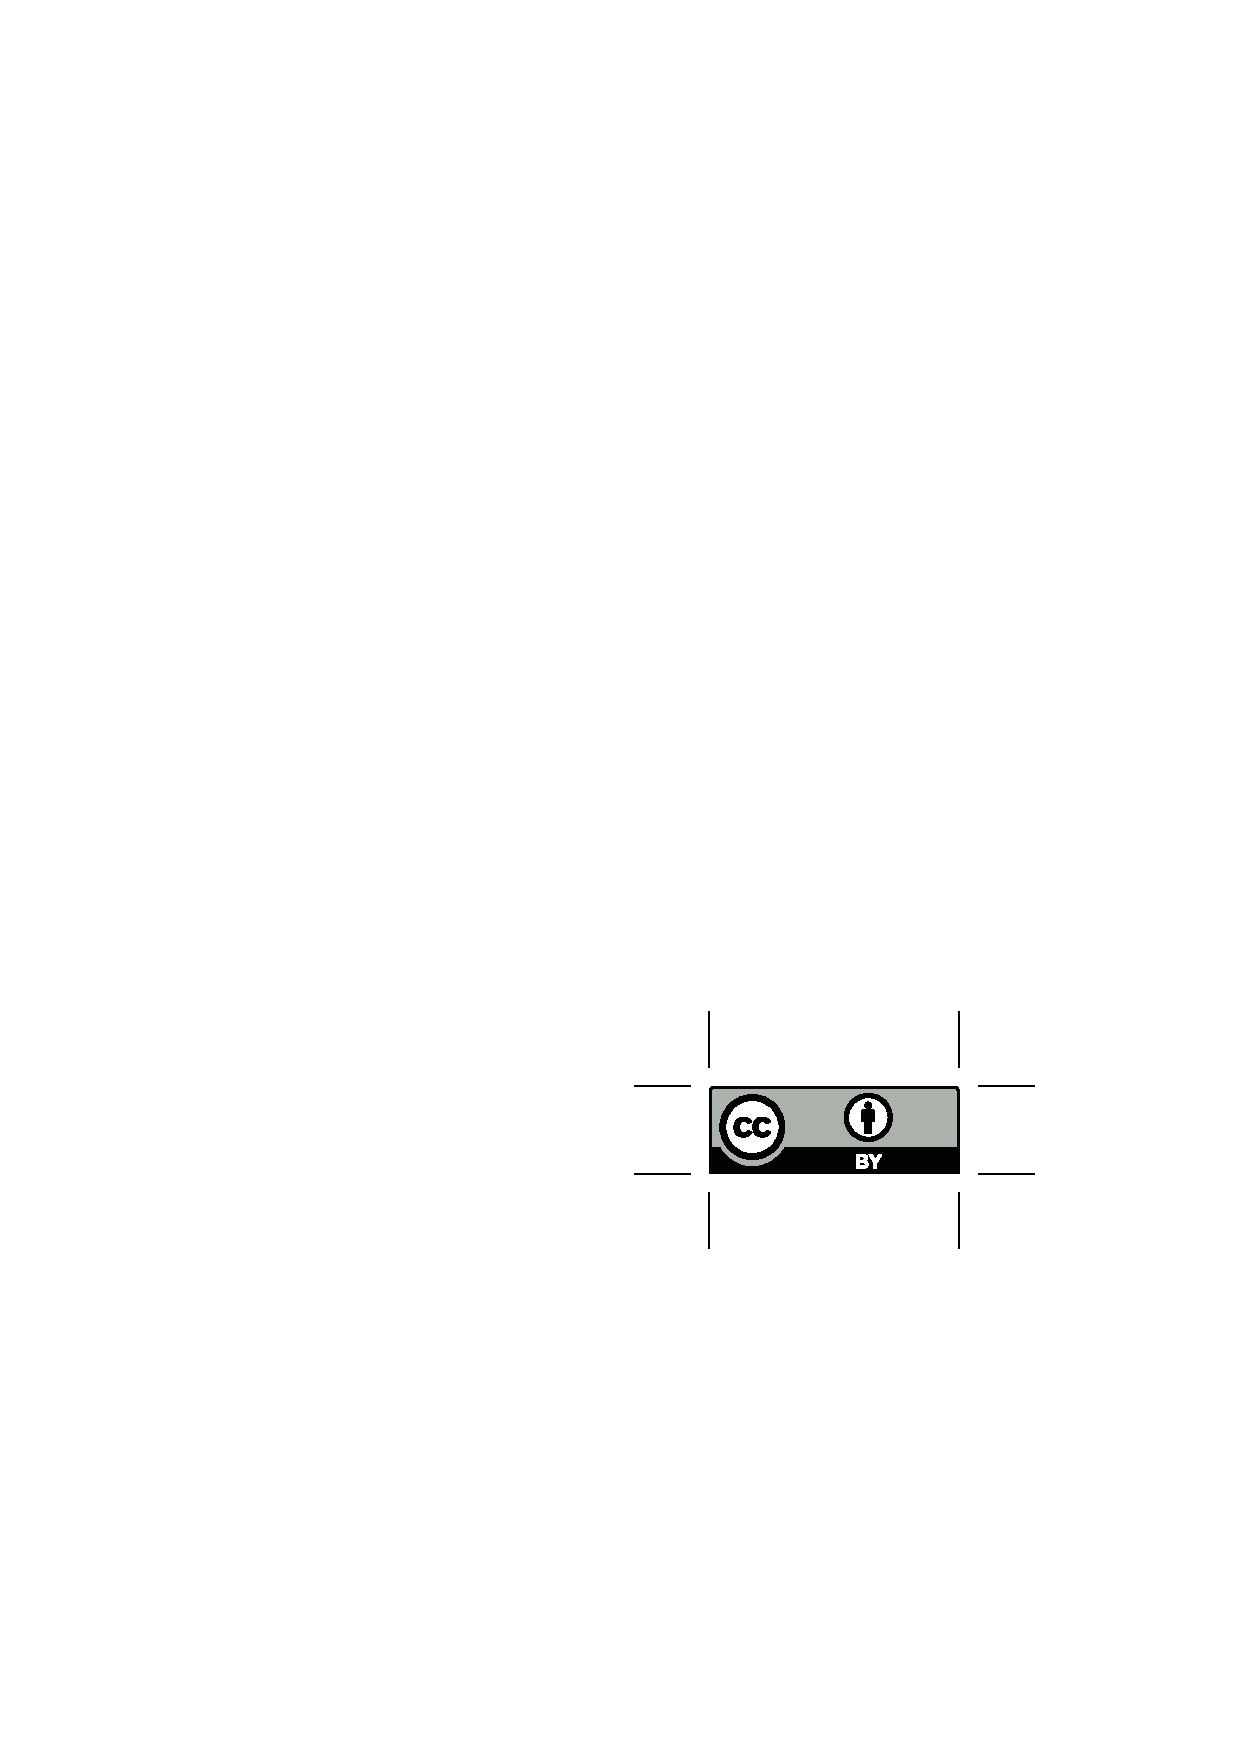
\includegraphics[height=14pt]{by} \\

{\tiny
This work is licensed under a
\href{http://creativecommons.org/licenses/by/4.0/}{Creative Commons Attribution 4.0 International License}.
}}

\begin{document}

\begin{frame}
  \titlepage
\end{frame}

\begin{frame} \frametitle{Big Idea: Algorithm Frameworks}
  \textbf{Algorithm framework:} an algorithm with modular parts that can be
    swapped in for different performance properties; or to solve different but
    related problems \stanza

  Example: hash tables are a framework, can swap in
  \begin{itemize}
    \item different collision resolution strategy (chaining, probing)
    \item different hash function (universal hash, linear congruential hash, etc.)
  \end{itemize}

  A framework generalizes several algorithm ideas into one pattern; ``chunking''
\end{frame}

\begin{frame} \frametitle{Big Idea: Iterative Pattern}
\begin{columns}
\begin{column}{0.5\textwidth}
Recall greedy pattern:
\begin{enumerate}
  \item initialize base-case result
  \item for each piece of input, update result
\end{enumerate}
\end{column}
\begin{column}{0.5\textwidth}
\textbf{Iterative pattern} (a.k.a. \emph{fixed-point algorithm}):
\begin{enumerate}
  \item initialize base-case result
  \item while result is not optimal:
  \begin{enumerate}
    \item improve result one step
  \end{enumerate}
\end{enumerate}
\end{column}
\end{columns}
\vspace{.5cm}
Both use a \emph{greedy heuristic}; iterative pattern makes a problem-wide decision.
\end{frame}

\begin{frame} \frametitle{Big Idea: Problem Reduction}
\emph{problem A reduces to problem B} $=$ can use an algorithm for B to do all the hard
work of solving problem A \\
$=$ A is easier than B (or tied) \stanza

Sometimes A, B are closely related (e.g. forward-sorting, reverse-sorting) \stanza

More interesting: problems seem completely unrelated (e.g. SAT, CLIQUE;
max-flow, bipartite matching)
\end{frame}

\begin{frame} \frametitle{Big Idea: Problem Duality}
\textbf{problem duality:} when the input/output mathematical definition of a
problem can be interpreted by humans in two (or more) very different ways
\begin{itemize}
  \item one algorithm can solve multiple problems with different ``stories''
  \item algorithms, computers, don't actually care what data values mean
  \item turns out max-flow and min-cut are two different stories for the same problem
  \item max-flow and min-cut are the \emph{dual of each other}
\end{itemize}
\end{frame}


\begin{frame} \frametitle{Link to Content Slides}

See Kevin Wayne's slides at Titanium

\end{frame}

\end{document}
